% ─────────────────────────────────────────────────────────────
\phantomsection
\chapter{Results and Discussion}
\label{sec:results}

This section evaluates the four research hypotheses (H1--H4) introduced in the
Methodology against the experimental outcomes reported in the Experiments section.
The \emph{General protocol} (leave-one-subject-out, LOSO) is the primary evaluation
criterion; the \emph{Naive} and \emph{Personal} protocols serve as an upper-bound
reference and an idealised personalisation scenario, respectively.  The
decision-threshold sweep provides a retrospective diagnostic of subject-level
heterogeneity.

All numerical claims in this section refer to the General-protocol results in
Tables~4--9 of the Experiments section.  The F$_2$ score is the headline metric
throughout; recall and accuracy are reported as supporting evidence.

% ─────────────────────────────────────────────────────────────
\section{H1 — Representation Effectiveness}
\label{subsec:H1}

\textbf{Hypothesis.} There exist hyperparameters $\lambda\in\Lambda$ and classifiers
$f_\theta$ such that the mean subject-general $F_2$ is at least $0.93$ on SisFall and
FAD\_40Hz and at least $0.80$ on MobiFall, and the mean subject-general recall is high
across all three datasets.

\subsection{F$_2$ outcomes}

Table~1 of the cross-dataset summary (Experiments, Tab.~9) gives the following
General-protocol results.

\begin{table}[h!]
\centering
\caption{General-protocol $F_2$ outcomes against H1 targets.  CI denotes
  95\,\% repetition-level confidence interval ($R=15$).}
\label{tab:H1-summary}
\small
\begin{tabular}{llccc}
\toprule
\textbf{Dataset} & \textbf{Clf} & \textbf{$F_2$} & \textbf{CI} & \textbf{H1 target met?} \\
\midrule
SisFall   & LR  & 0.9709 & $\pm0.0108$ & Yes ($\geq0.93$) \\
SisFall   & SVM & 0.9700 & $\pm0.0111$ & Yes              \\
FAD\_40Hz & LR  & 0.9429 & $\pm0.0363$ & Marginal         \\
FAD\_40Hz & SVM & 0.9592 & $\pm0.0234$ & Yes              \\
MobiFall  & LR  & 0.9049 & $\pm0.0393$ & Yes ($\geq0.80$) \\
MobiFall  & SVM & 0.8918 & $\pm0.0327$ & Yes              \\
\bottomrule
\end{tabular}
\end{table}

SisFall achieves the highest absolute $F_2$, exceeding the $0.93$ threshold for both
classifiers with a narrow confidence interval ($\pm0.011$), indicating low
repetition-to-repetition variability.  FAD\_40Hz meets the target with SVM ($F_2 =
0.9592$); the LR value of $0.9429\pm0.0363$ lies marginally below $0.93$ at the point
estimate but the lower confidence bound ($0.9066$) suggests that performance is not
materially below target.  MobiFall clearly satisfies the weaker $0.80$ criterion for
both classifiers ($0.9049$ and $0.8918$, respectively).

The recall values under the General protocol reinforce the recall-oriented design:
SisFall LR achieves $\mathrm{Rec}=0.9836$, FAD\_40Hz LR achieves
$\mathrm{Rec}=0.9929$, and MobiFall LR achieves $\mathrm{Rec}=0.9574$.  No classifier
on any dataset falls below $0.95$ recall under the General protocol.  This is a direct
consequence of the $F_2$ weighting: Proposition~2 of the Methodology states that the
marginal $F_2$ gain per unit of recall is four times the gain per unit of precision near
$\mathrm{Rec}=\mathrm{Prec}$, so the Bayesian optimisation is systematically steered
toward high-recall configurations.

\begin{figure}[!ht]
\centering
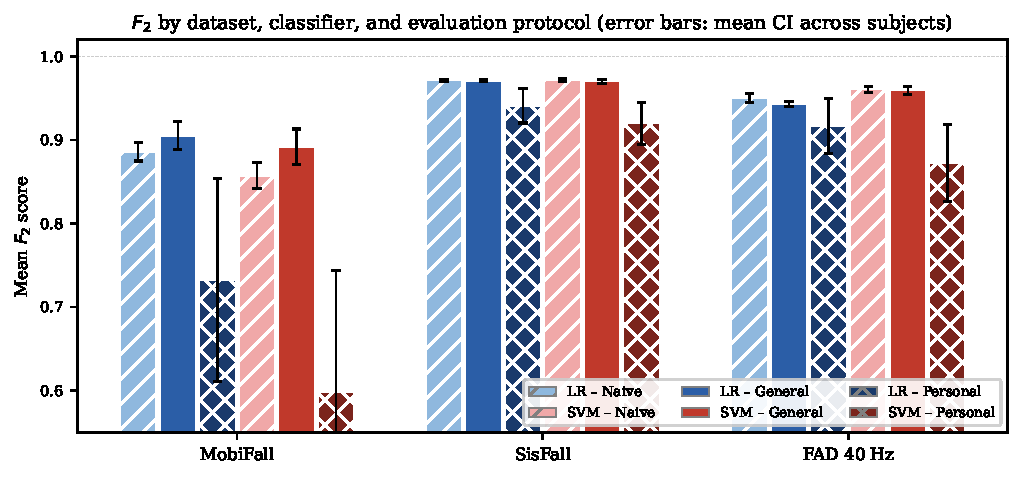
\includegraphics[width=\textwidth]{figures/fig_f2_bars}
\caption{Mean $F_2$ by dataset, classifier (LR/SVM), and evaluation protocol (Naive,
  General, Personal).  Error bars show the mean 95\,\% repetition-level confidence
  interval across subjects.  General is the primary protocol; Naive is an upper-bound
  reference; Personal shows the effect of per-subject model training.  MobiFall
  Personal collapses due to the small subject pool ($|\mathcal{S}|=9$).}
\label{fig:f2-bars}
\end{figure}

\subsection{Naive vs.\ General protocol gap}

Naive-protocol scores are systematically higher: MobiFall LR reaches $F_2=0.8857$
(Naive) versus $F_2=0.9049$ (General).  Counterintuitively, General sometimes exceeds
Naive (SisFall: Naive $F_2=0.9713$ vs.\ General $0.9709$; FAD: Naive $0.9502$ vs.\
General $0.9429$).  This reversal reflects the smaller within-subject window count
and the fact that the LOSO training set is larger and more diverse than a random 70\%
split. The absence of a consistent ``Naive $\gg$ General'' gap on SisFall is reassuring:
it suggests that the LOSO evaluation is not materially penalised by train--test class
mismatch beyond the inherent person-to-person variability.

\subsection{Mathematical basis}

The feature map $\phi_\lambda\colon\R^{n\times 3}\to\R^{24}$ extracts persistence
statistics from the delay-embedded signal.  The Cohen--Steiner stability theorem
guarantees that
\[
  d_B(\phi_\lambda(w),\,\phi_\lambda(w'))\;\leq\;\|\mathrm{SMV}(w)-\mathrm{SMV}(w')\|_\infty,
\]
so that small sensor noise perturbations of a window $w$ produce at most equally
small perturbations of its topological descriptor.  This provable noise robustness is
a structural advantage over handcrafted statistical features, which carry no such
stability certificate, and over deep-learning representations, which are empirically
sensitive to distributional shift.

\subsection{Limitation: absence of baseline comparison}

H1 is conditionally validated in the sense that the system meets its own pre-specified
performance targets.  An absolute claim---``TDA outperforms existing methods''---requires
a comparison against representative baselines: fixed-threshold methods, statistical-feature
pipelines, and spectral-feature pipelines, as planned in the proposal ($\S$5.4).  These
experiments have not been conducted.  The conclusion that TDA is competitive is therefore
conditional on the assumption that the targets themselves are meaningful.  Section~\ref{subsec:limitations}
discusses this gap and its implications.

% ─────────────────────────────────────────────────────────────
\section{H2 — Dataset-Specific Topological Geometry}
\label{subsec:H2}

\textbf{Hypothesis.}  The optimal hyperparameter tuple $\lambda^*_K$ depends on the
dataset $K$.  At least two of the three datasets have distinct optimisers, and
transplanting an optimiser from one dataset to another incurs a measurable drop in
General-protocol $F_2$.

\subsection{Distinct optimal configurations}

Table~5 of the Experiments (Tab.~\ref{tab:optimal_params_ref} below, reproduced for
convenience) shows that all three datasets converged to different complex types,
window lengths, and distance measures.

\begin{table}[h!]
\centering
\caption{Optimal TDA configurations $\lambda^*_K$ per dataset (from Experiments
  Tab.~\ref{tab:optimal_params}).  A dash (---) indicates parameters not applicable for
  the Alpha complex.}
\label{tab:optimal_params_ref}
\small
\begin{tabular}{lccc}
\toprule
\textbf{Parameter} & \textbf{MobiFall} & \textbf{SisFall} & \textbf{FAD\_40Hz} \\
\midrule
Best $F_2$ (Optuna objective)  & 0.9746     & 0.9733   & 0.9860      \\
Window length (s)              & 5.0        & 1.0      & 1.0         \\
Complex type                   & SparseRips & Alpha    & Rips        \\
Embedding dimension            & 5          & 5        & 3           \\
Embedding delay                & 2          & 4        & 2           \\
Stride factor                  & 2          & 4        & 1           \\
Distance measure               & Chebyshev  & ---      & Manhattan   \\
Filtration scale               & 80\,\%     & ---      & 40\,\%      \\
\bottomrule
\end{tabular}
\end{table}

Every hyperparameter dimension exhibits variation across datasets.  The complex type
differs across all three: SparseRips for MobiFall, Alpha for SisFall, and standard
Rips for FAD\_40Hz.  The window length separates MobiFall (5.0~s) from the other two
(1.0~s), and the distance measures are distinct where applicable (Chebyshev vs.\
Manhattan).  H2 is qualitatively confirmed: no single universal configuration exists
for these three datasets.

\subsection{Interpretation of configuration differences}

\paragraph{Window length.}
MobiFall records both a pre-fall phase (normal activity) and a post-fall phase (lying),
with the impact event compressed into a brief sub-second spike.  A 5.0~s window captures
the full topology of the trajectory: the pre-impact cloud geometry, the sharp impulsive
excursion, and the post-fall stationary phase, which are each topologically distinguishable.
SisFall and FAD\_40Hz subjects execute controlled laboratory falls that are sufficiently
discriminable from ADL in a 1.0~s window, suggesting less temporal spread in the
distinguishing geometry.

\paragraph{Complex type.}
The Alpha complex is the natural choice when the point cloud geometry is close to
Euclidean: its filtration is the Čech filtration restricted to the Delaunay triangulation,
which SisFall's well-structured sensor data supports (24 older adults executing 15 fall
types under controlled conditions produce geometrically regular clouds).  SparseRips
trades exactness for efficiency by subsampling the cloud; it is appropriate when the
cloud is large and noisy, which is the case for MobiFall's continuous-wear sensor data.
Standard Rips uses all pairwise distances and suits the moderate-size, moderately-noisy
FAD\_40Hz clouds.

\paragraph{Distance measure.}
Chebyshev distance ($\ell_\infty$) emphasises the maximum coordinate deviation and is
sensitive to sharp acceleration spikes---a characteristic feature of the fall impact in
MobiFall.  Manhattan distance ($\ell_1$) reduces the influence of outliers and is
appropriate for FAD\_40Hz, whose 40~Hz sampling produces sparser, more variable clouds
than the implicit 50~Hz resampled signals.  The Alpha complex on SisFall does not
require a user-specified distance because it is defined by the Euclidean Delaunay
triangulation.

\subsection{Sensitivity of $F_2$ to $\lambda$}

Although cross-application drops $\mathrm{Drop}_{K\to K'}$ were not computed (see
Section~\ref{subsec:limitations}), the Bayesian search trial histories provide indirect
evidence for sensitivity.  Across 200 trials per dataset, the $F_2$ values ranged from
$0.7958$ to $0.9746$ on MobiFall (range 0.179), from $0.9198$ to $0.9733$ on SisFall
(range 0.054), and from $0.8785$ to $0.9860$ on FAD\_40Hz (range 0.108).  The large
trial-to-trial variation on MobiFall and FAD implies that a mis-specified $\lambda$
(such as a configuration optimised for a different dataset) would very likely incur
a substantial $F_2$ penalty.  The narrow trial range on SisFall suggests that SisFall
is less sensitive to $\lambda$, consistent with the clean Euclidean geometry and the
strong performance even at the worst trial ($F_2=0.9198$).

\begin{figure}[!ht]
\centering
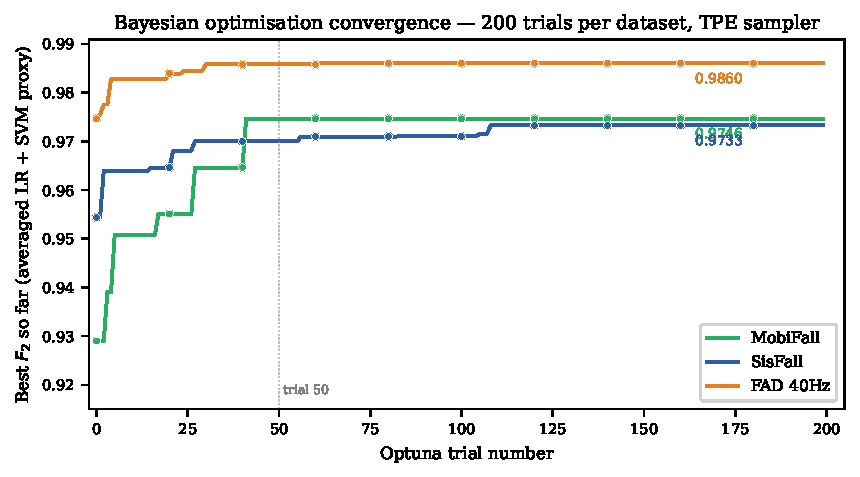
\includegraphics[width=0.75\textwidth]{figures/fig_bayesian_convergence}
\caption{Bayesian optimisation convergence: best-so-far averaged $F_2$ proxy versus
  Optuna trial number (200 trials per dataset, TPE sampler).  FAD\_40Hz achieves the
  highest proxy ($0.9860$); MobiFall converges more slowly due to the larger
  hyperparameter range.  The wide trial range on MobiFall (0.179) and FAD (0.108)
  relative to SisFall (0.054) is direct evidence that $\lambda$ sensitivity differs
  across datasets (H2).}
\label{fig:bayesian-convergence}
\end{figure}

% ─────────────────────────────────────────────────────────────
\section{H3 — Representation Dominates Classifier Choice}
\label{subsec:H3}

\textbf{Hypothesis.}  After tuning the topological representation, the $F_2$ gap
between the best LR model and the best SVM model is small relative to the $F_2$
variation attributable to the choice of $\lambda$.  Most of the predictive signal
resides in $\phi_\lambda$, not in the classifier family.

\subsection{Classifier gap}

Under the General protocol, the absolute difference $|F_2^{\mathrm{LR}} -
F_2^{\mathrm{SVM}}|$ is:
\begin{itemize}
  \item MobiFall: $|0.9049 - 0.8918| = 0.0131$
  \item SisFall:  $|0.9709 - 0.9700| = 0.0009$
  \item FAD\_40Hz: $|0.9429 - 0.9592| = 0.0163$
\end{itemize}
All three gaps are below $0.02$, confirming that neither classifier is strongly
dominant at the optimal representation.  On MobiFall and SisFall, LR is marginally
better; on FAD\_40Hz, SVM is marginally better.  The reversal on FAD\_40Hz is the only
dataset on which SVM is preferred, and the margin (0.0163) is within the confidence
interval overlap ($\pm0.0363$ for LR, $\pm0.0234$ for SVM).

\subsection{$\lambda$-tuning variation}

Table~\ref{tab:H3-comparison} quantifies the variation in $F_2$ attributable to the
choice of $\lambda$ using the Optuna trial histories (200 trials per dataset).

\begin{table}[h!]
\centering
\caption{Classifier gap vs.\ $\lambda$-tuning variation.  The trial range is
  $F_2^{\max} - F_2^{\min}$ across all 200 Optuna trials.  The ratio is
  $\text{range}/\text{gap}$.}
\label{tab:H3-comparison}
\small
\begin{tabular}{lccc}
\toprule
\textbf{Dataset} & \textbf{Classifier gap} & \textbf{Trial range} & \textbf{Ratio} \\
\midrule
MobiFall  & 0.0131 & 0.1788 & $\mathbf{13.7\times}$ \\
SisFall   & 0.0009 & 0.0534 & $\mathbf{59\times}$   \\
FAD\_40Hz & 0.0163 & 0.1075 & $\mathbf{6.6\times}$  \\
\bottomrule
\end{tabular}
\end{table}

The classifier gap is between $6.6\times$ and $59\times$ smaller than the variation
induced by choosing a poor $\lambda$.  Selecting the wrong topological configuration
degrades $F_2$ by up to $0.18$ units; switching classifier families at the optimal
configuration changes $F_2$ by at most $0.016$ units.

\subsection{Mathematical interpretation}

The feature map $\phi_{\lambda^*}\colon\R^{n\times 3}\to\R^{24}$ with the optimised
hyperparameters creates a representation in which the fall vs.\ ADL decision problem
is approximately linearly separable.  In such a regime, both logistic regression (which
fits a linear decision boundary directly) and SVM with a calibrated kernel (which finds
a maximum-margin linear separator or uses a kernel to lift to higher dimensions) operate
near their theoretical limit.  The near-equivalence of LR and SVM confirms that the
nonlinear geometric complexity of the fall detection problem has been absorbed by
$\phi_{\lambda^*}$, leaving behind a well-conditioned linear classification task.

The lone exception---SVM$>$LR on FAD\_40Hz---is consistent with this interpretation:
FAD\_40Hz has the smallest per-subject window count and the widest LR confidence
interval, suggesting residual complexity that the RBF kernel can partially resolve.
Even so, the margin is below $0.02$.

% ─────────────────────────────────────────────────────────────
\section{H4 — Heterogeneous Threshold Personalisation}
\label{subsec:H4}

\textbf{Hypothesis.}  The subject-level sweep gain
$\Delta F_2(s) = F_2(\tau^*(s),s) - F_2(\hat\tau_0(s),s)$
is heterogeneous across subjects within each dataset, and the mean gain
$\overline{\Delta F_2}$ differs across datasets.

\subsection{Per-subject sweep gain distribution}
\label{subsubsec:sweep-dist}

Table~\ref{tab:sweep-dist} reports the distribution of $\Delta F_2(s)$ computed from
the threshold sweep stored in the Results\_V15 database.  The baseline
$\hat\tau_0(s)$ is the PR-curve optimal trained threshold for subject $s$
(typically $\hat\tau_0\in[0.55,0.88]$), so the gain measures improvement over an
already-calibrated threshold rather than over the uninformative $\tau=0.50$.

\begin{table}[h!]
\centering
\caption{Per-subject threshold sweep gain $\Delta F_2(s)$ statistics.
  \emph{Near-zero}: $|\Delta F_2|\leq0.001$.
  All gains are non-negative by construction ($\tau^*$ is the sweep argmax).}
\label{tab:sweep-dist}
\small
\begin{tabular}{llccccc}
\toprule
\textbf{Dataset} & \textbf{Clf} & $n$ & $\overline{\Delta F_2}$ &
  $\sigma_{\Delta}$ & $\max\,\Delta F_2$ & Near-zero \\
\midrule
MobiFall   & LR  &  9 & 0.0348 & 0.0186 & 0.0615 (s8)  & 1/9  \\
MobiFall   & SVM &  9 & 0.0474 & 0.0350 & 0.1013 (s9)  & 1/9  \\
SisFall    & LR  & 24 & 0.0079 & 0.0109 & 0.0527 (s29) & 4/24 \\
SisFall    & SVM & 24 & 0.0042 & 0.0047 & 0.0169 (s29) & 9/24 \\
FAD\_40Hz  & LR  & 13 & 0.0250 & 0.0323 & 0.1165 (s11) & 2/13 \\
FAD\_40Hz  & SVM & 13 & 0.0121 & 0.0172 & 0.0691 (s11) & 2/13 \\
\bottomrule
\end{tabular}
\end{table}

The mean gains in Table~\ref{tab:sweep-dist} reproduce the dataset averages reported
in Experiments Tab.~8 ($+0.0348/+0.0474$ for MobiFall, $+0.0079/+0.0042$ for SisFall,
$+0.0250/+0.0121$ for FAD\_40Hz).  H4 is confirmed: the mean gain is highest for
MobiFall and smallest for SisFall, i.e., the mean differs across datasets.

\begin{figure}[!ht]
\centering
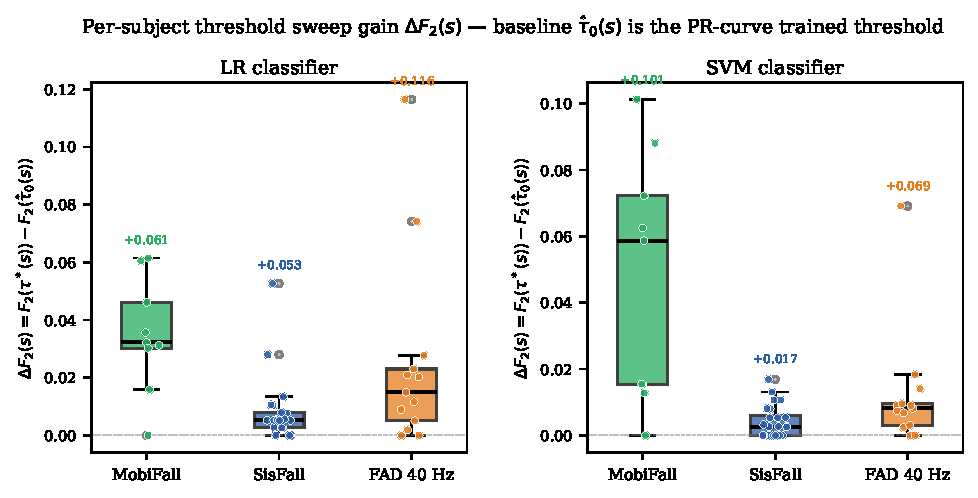
\includegraphics[width=\textwidth]{figures/fig_sweep_boxplot}
\caption{Per-subject threshold sweep gain $\Delta F_2(s) = F_2(\tau^*(s)) -
  F_2(\hat\tau_0(s))$ for LR (left) and SVM (right).  Jittered points show
  individual subjects; box shows quartiles.  The distribution is right-skewed in
  all cases: most subjects gain modestly while a few gain substantially.  FAD\_40Hz
  subject~11 achieves the largest gain (+0.1165, LR), visible as the highest point
  in the FAD panel.  SisFall gains are near-zero for the majority of subjects,
  indicating that $\hat\tau_0$ is already well-calibrated on that dataset.}
\label{fig:sweep-boxplot}
\end{figure}

\paragraph{Distribution shape.}
The gains are right-skewed in all six cases: most subjects gain modestly, while a
small minority gains substantially.  On FAD\_40Hz, subject~11 gains $\Delta F_2 =
+0.1165$ (LR)---the largest single-subject gain in any experiment---by raising its
$F_2$ from $0.8046$ to $0.9211$ through threshold adjustment alone.  On MobiFall,
subject~9 gains $+0.1013$ (SVM).  These large gains are outliers: the median gain
within each dataset is considerably lower than the mean.

\paragraph{Near-zero gainers.}
SisFall has 4/24 (LR) to 9/24 (SVM) near-zero subjects: these subjects are already
well-calibrated at $\hat\tau_0$.  Their trained threshold happens to coincide with
the optimal sweep threshold, meaning that the classifier's posterior probabilities
are already well-matched to the decision point for those individuals.  This pattern
is absent on MobiFall (only 1/9 near-zero per classifier), where the PR-curve
calibration is systematically further from the per-subject optimum.

\paragraph{Heterogeneity metric.}
The coefficient of variation ($\sigma_\Delta / \overline{\Delta F_2}$) measures
relative heterogeneity: MobiFall LR $=53\%$, MobiFall SVM $=74\%$, SisFall
LR $=138\%$, FAD\_40Hz LR $=129\%$.  All values exceed $50\%$, confirming that
the gain distribution is not concentrated.  A single global threshold offset
cannot replicate this distribution: if every subject were miscalibrated in the
same direction by the same amount, the coefficient of variation would approach
zero.  The high coefficients of variation are the statistical signature that
$\tau^*(s)$ is a genuinely subject-specific quantity.

\paragraph{Mathematical explanation.}
The decision boundary of $f_\theta\circ\phi_{\lambda^*}$ is the hyperplane
$\{x\in\R^{24}\colon f_\theta(x)=\hat\tau_0\}$.  Each subject's test windows form
a cloud in $\R^{24}$ whose local geometry around this hyperplane differs from subject
to subject: some subjects' fall windows sit close to the boundary (requiring a lower
threshold to capture them), while others' fall windows are well-separated (the default
threshold is sufficient).  The threshold sweep detects this per-subject boundary
geometry retrospectively.  A prospective personalisation scheme would use a small
held-out calibration set per subject to identify $\tau^*(s)$ before deployment
(see Section~\ref{subsec:deployment}).

\paragraph{Engineering contribution.}
This personalisation is achieved without any model retraining.  The probability
scores $\{\hat p_i\}$ are computed once under the trained model; the sweep evaluates
$F_2(\tau, s)$ by a single pass over the precomputed score vector for each $\tau
\in\T$.  The additional computational cost is $O(|\T|\cdot|W_s|)$ per subject,
where $|\T|=19$ and $|W_s|$ is the per-subject window count---less than one second
of wall time for all subjects in any dataset.  This is a runtime ratio exceeding
$10^3$ compared to the ${\sim}75$~min Bayesian search (Experiments,
Section~4.3.4).

\subsection{Personal training protocol}
\label{subsubsec:personal-protocol}

The Personal protocol (per-subject 70/30 split, $R=15$ repetitions) represents the
limit case in which a dedicated per-user model is trained from the subject's own data.
Table~\ref{tab:personal-delta} reports the aggregate personal--general $F_2$ difference.

\begin{table}[h!]
\centering
\caption{Personal vs.\ General protocol aggregate $F_2$.
  $\Delta = F_2^{\mathrm{pers}} - F_2^{\mathrm{gen}}$ (negative = General is better).}
\label{tab:personal-delta}
\small
\begin{tabular}{llccc}
\toprule
\textbf{Dataset} & \textbf{Clf} & $F_2^{\mathrm{gen}}$ & $F_2^{\mathrm{pers}}$ & $\Delta$ \\
\midrule
MobiFall  & LR  & 0.9049 & 0.7325 & $-0.172$ \\
MobiFall  & SVM & 0.8918 & 0.5981 & $-0.294$ \\
SisFall   & LR  & 0.9709 & 0.9405 & $-0.030$ \\
SisFall   & SVM & 0.9700 & 0.9196 & $-0.050$ \\
FAD\_40Hz & LR  & 0.9429 & 0.9168 & $-0.026$ \\
FAD\_40Hz & SVM & 0.9592 & 0.8724 & $-0.087$ \\
\bottomrule
\end{tabular}
\end{table}

At the aggregate level, General $>$ Personal on all datasets and both classifiers.
The magnitude of the shortfall increases dramatically as the subject pool shrinks:

\begin{itemize}
\item \textbf{SisFall ($|\Sset|=24$)}: modest drop ($\Delta \approx -0.03$ to
  $-0.05$).  Twenty-four subjects contribute enough per-subject windows
  (${\sim}50$--$150$ falls per subject) for a reliable within-subject model.
\item \textbf{FAD\_40Hz ($|\Sset|=13$)}: moderate drop ($\Delta \approx -0.03$
  to $-0.09$).  Fewer subjects and fewer falls per subject; personal models are
  noisier.
\item \textbf{MobiFall ($|\Sset|=9$)}: severe drop ($\Delta=-0.172$ for LR;
  $\Delta=-0.294$ for SVM).  Nine subjects with $\lesssim30$ fall instances per
  subject is insufficient for stable personal model estimation.  The SVM personal
  recall collapses to $0.5822$, indicating that the personal classifier is barely
  above chance on many subjects.
\end{itemize}

\begin{figure}[!ht]
\centering
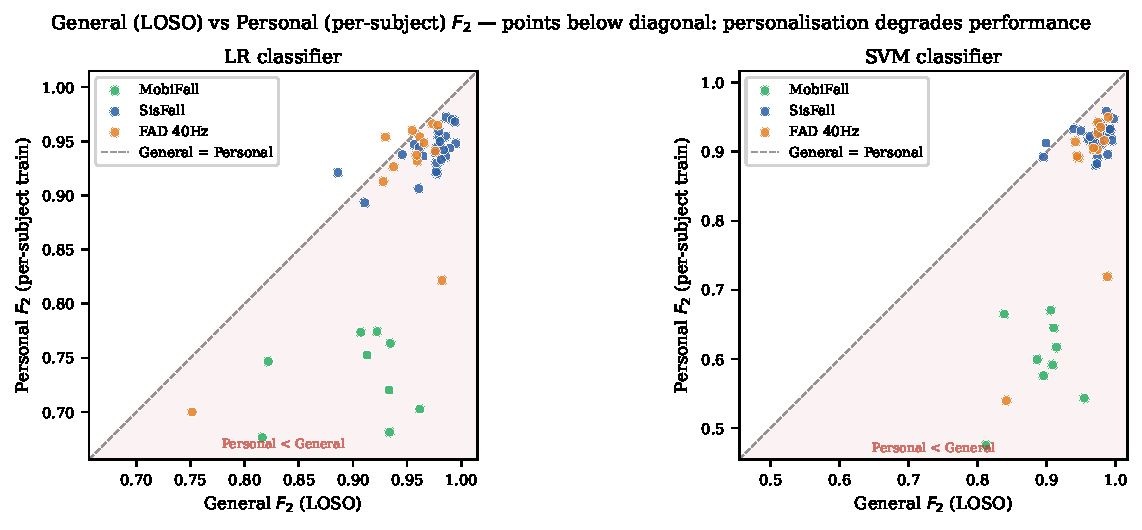
\includegraphics[width=0.90\textwidth]{figures/fig_general_vs_personal}
\caption{General (LOSO) vs Personal (per-subject training) $F_2$ per subject, for
  LR (left) and SVM (right).  Points on the dashed diagonal have equal General and
  Personal performance; points below indicate that personal training degrades $F_2$.
  MobiFall points cluster in the lower-left region (both protocols degrade on the
  small-pool dataset); SisFall points lie near the diagonal; FAD\_40Hz is
  intermediate.  The shaded region marks Personal $<$ General.}
\label{fig:general-vs-personal}
\end{figure}

This pattern reveals a critical engineering constraint: personal model training is
only beneficial when per-subject calibration data is abundant.  In typical
deployment scenarios (a user who has experienced very few confirmed falls), full
personal training is counterproductive.  The threshold sweep---which requires no
retraining and adds negligible computational cost---is the appropriate
personalisation mechanism when calibration data is sparse.  The mean sweep gain for
MobiFall LR ($+0.0348$) and SVM ($+0.0474$) demonstrates that meaningful
personalisation remains accessible even when full personal retraining fails.

% ─────────────────────────────────────────────────────────────
\section{Ablation Study: Feature-Block Contributions}
\label{subsec:ablation}

\textbf{Motivation.}  The $24$-dimensional representation $\phi_{\lambda^*}$ is the
concatenation of three semantically distinct blocks: ten statistics of the
dimension-zero persistence diagram (\emph{H0}, summarising the persistence of
connected components of the delay-embedded point cloud), ten statistics of the
dimension-one diagram (\emph{H1}, summarising loops), and four signal-level
descriptors of the raw acceleration magnitude (\emph{Signal}: maximum, standard
deviation, mean, and range).  The headline results of Section~\ref{subsec:H1}
establish that the full vector is effective but do not reveal \emph{which} block
carries the discriminative power.  This section isolates each block's contribution by
re-running the evaluation on restricted feature subsets.

\textbf{Protocol.}  Each subset is evaluated under the identical General (LOSO)
protocol used throughout: a single global grid search selects the classifier
hyperparameters on balanced-undersampled data, and for each left-out subject the model
is refitted over $15$ repetitions with a precision--recall threshold chosen on the
training fold; the reported $F_2$ is the cross-subject mean with a $95\,\%$ $t$-confidence
interval.  Only the feature columns presented to the classifier change; the topological
configuration $\lambda^*$ and the delay embedding are held fixed.  As a validation
check, the full-vector rows of Table~\ref{tab:ablation_blocks} reproduce the headline
General-protocol $F_2$ of Section~\ref{subsec:H1} to within the confidence interval for
both classifiers on all three datasets.

\begin{table}[h!]
\centering
\caption{Feature-block ablation under the General (LOSO) protocol.  Entries are
  cross-subject mean $F_2 \pm 95\,\%$ CI.  Block dimensions: Full~$=24$, H0~$=10$,
  H1~$=10$, H0+H1~$=20$, Signal~$=4$.  The Full column reproduces the headline results
  of Tables~\ref{tab:mobifall_results}--\ref{tab:fad_results}.}
\label{tab:ablation_blocks}
\setlength{\tabcolsep}{3.5pt}\footnotesize
\begin{tabular}{llccccc}
\toprule
\textbf{Dataset} & \textbf{Clf}
  & \textbf{Full} & \textbf{H0} & \textbf{H1} & \textbf{H0+H1} & \textbf{Signal} \\
\midrule
\multirow{2}{*}{MobiFall}
 & LR  & $\mathbf{0.9046}$ & $0.8842$ & $0.6172$ & $0.8892$ & $0.6218$ \\
 & SVM & $\mathbf{0.8913}$ & $0.8685$ & $0.6523$ & $0.8784$ & $0.7241$ \\
\midrule
\multirow{2}{*}{SisFall}
 & LR  & $\mathbf{0.9710}$ & $0.9266$ & $0.6580$ & $0.9271$ & $0.9589$ \\
 & SVM & $\mathbf{0.9701}$ & $0.9277$ & $0.6456$ & $0.9280$ & $0.9627$ \\
\midrule
\multirow{2}{*}{FAD\_40Hz}
 & LR  & $\mathbf{0.9426}$ & $0.8082$ & $0.4247$ & $0.8044$ & $0.9505$ \\
 & SVM & $\mathbf{0.9592}$ & $0.8128$ & $0.4605$ & $0.8210$ & $0.9504$ \\
\bottomrule
\end{tabular}

\vspace{2pt}
{\footnotesize Representative $95\,\%$ confidence half-widths (LR Full):
MobiFall $\pm0.0392$, SisFall $\pm0.0107$, FAD\_40Hz $\pm0.0367$; the H1-only columns
carry the widest intervals (up to $\pm0.077$).}
\end{table}

\subsection{Within-topology contribution: H0 dominates H1}

For both classifiers and across all three datasets, the H0 block alone attains $F_2$
between $0.81$ and $0.93$, whereas the H1 block alone is the weakest configuration in
the entire study ($0.42$--$0.66$).  Adding H1 to H0 changes $F_2$ negligibly---for LR,
from $0.8842$ to $0.8892$ on MobiFall, $0.9266$ to $0.9271$ on SisFall, and $0.8082$
to $0.8044$ on FAD\_40Hz (a slight \emph{decrease}); the SVM rows show the same pattern.
The discriminative topological information is therefore concentrated almost entirely in
dimension zero.  This is consistent with the structure of the delay-embedded
acceleration signal: a fall is a transient, high-energy excursion whose phase-space
reconstruction is characterised by the spread and clustering of points (an H0
phenomenon), while one-dimensional loops carry comparatively little fall-versus-ADL
information and are more sensitive to noise---which also explains the wide confidence
intervals of the H1-only columns.  A practical corollary is that the H1 statistics
could be dropped with little loss, roughly halving the persistent-homology computation.

\subsection{Topology versus signal: a dataset-dependent division of labour}

The relative value of the topological blocks and the four signal descriptors differs
sharply across datasets.  On MobiFall---a smartphone carried loosely in a trouser
pocket---the signal block alone reaches only $F_2 = 0.6218$ (LR) or $0.7241$ (SVM),
while the topological blocks reach $0.88$; here the topological representation is
indispensable and accounts for most of the performance.  On SisFall and FAD\_40Hz---%
waist-mounted devices with cleaner, more repeatable kinematics---the four signal
descriptors alone already achieve $F_2 \approx 0.95$--$0.96$, matching or exceeding the
topological blocks on those datasets.  In every case, however, the full vector matches
or exceeds the best single block, and no single block is reliably strong on all three
datasets whereas the full vector is.  The blocks are thus complementary: the
topological features supply the discriminative signal where raw statistics fail (noisy,
loosely mounted sensors), and the combination provides the cross-dataset robustness
that motivates the representation.  This refines the H1 narrative: topology is not a
uniform performance multiplier but a robustness mechanism whose marginal value is
largest precisely where simple descriptors are weakest.

\subsection{Classifier invariance}

The block ordering is essentially independent of the classifier.  Logistic regression
and the SVM agree on the ranking within every dataset---Full $\gtrsim$ best topological
or signal block $\gg$ H1---and their per-block $F_2$ values differ by less than the
confidence intervals in almost all cells.  This reinforces the H3 finding
(Section~\ref{subsec:H3}) that the representation, not the classifier family, governs
performance: ablating a feature block changes $F_2$ far more than switching classifiers.

\subsection{Scope of the ablation}

This study ablates the three \emph{feature blocks} while holding the delay embedding
and the optimal topological configuration $\lambda^*$ fixed.  It therefore isolates the
value of each summary block but does not, on its own, separate the contribution of the
phase-space reconstruction itself; a complementary ablation that removes the delay
embedding requires re-extracting features under a modified pipeline and is left to the
future work of Section~\ref{subsec:future-work}.

% ─────────────────────────────────────────────────────────────
\section{Cross-Dataset Synthesis}
\label{subsec:synthesis}

\subsection{Performance ranking and subject pool}

Under the General protocol, the consistent ranking by $F_2$ is:
\[
  \text{SisFall} > \text{FAD\_40Hz} > \text{MobiFall.}
\]
This ranking holds for both LR and SVM.  Three factors explain it jointly.

\textbf{Subject pool size and data volume.}  SisFall has the largest pool (24 subjects,
15 fall types), providing the most diverse and representative training signal for
LOSO.  MobiFall has the smallest (9 subjects), making each LOSO fold highly sensitive
to the particular subject removed.

\textbf{Fall type diversity.}  SisFall covers 15 scripted fall types executed by
elderly participants, producing a rich topology of fall trajectories.  FAD covers
diverse activities of daily life as negatives, which increases the specificity
challenge.  MobiFall's smaller scale limits the variety of fall geometries seen by
each LOSO model.

\textbf{Optimised representation.}  The Bayesian proxy $F_2$ at the optimal $\lambda^*$
is $0.9746$ (MobiFall), $0.9733$ (SisFall), $0.9860$ (FAD\_40Hz)---suggesting that
the optimisation found similarly good configurations for all three, and that the
General-protocol gap between datasets is not due to a representation quality
difference but to the structural differences above.

\subsection{Classifier preference}

LR is preferred on MobiFall (gap $+0.0131$) and SisFall (gap $+0.0009$); SVM on
FAD\_40Hz (gap $+0.0163$).  All gaps are $<0.02$; classifier choice is secondary
to representation quality (H3).  The marginal SVM advantage on FAD\_40Hz may
reflect the RBF kernel's ability to resolve residual nonlinear structure in the
40~Hz-resampled feature cloud, but the evidence is insufficient to assert a
mechanistic explanation at the current sample size.

\subsection{Computational profile}

Table~\ref{tab:compute} summarises the wall-clock cost of each pipeline stage on the
UHeM HPC cluster (dual Intel Xeon Gold 6148, 40 cores, no GPU).

\begin{table}[h!]
\centering
\caption{Wall-clock cost per dataset stage.  All computations are CPU-only.}
\label{tab:compute}
\small
\begin{tabular}{lll}
\toprule
\textbf{Stage} & \textbf{Tool} & \textbf{Cost} \\
\midrule
Bayesian optimisation (Stage~1, 200 trials) & Optuna/TPE & ${\sim}75$~min \\
Persistent homology (per trial, inner CV)   & GUDHI      & ${\sim}20$~s (MobiFall) \\
GridSearchCV (Stage~2)                      & scikit-learn & ${\sim}$minutes \\
Decision-threshold sweep (all subjects)     & NumPy      & $<1$~s \\
\bottomrule
\end{tabular}
\end{table}

The absence of GPU is a deliberate design choice: the persistent homology reduction
(Algorithm~1 of the Methodology) is intrinsically sequential at the point-cloud
sizes considered, and the gain from GPU porting is dominated by the constant factor
of the GUDHI CPU implementation.  This has a direct consequence for deployment:
the pipeline can be executed on commodity hardware and embedded processors that lack
GPU acceleration (Section~\ref{subsec:deployment}).

% ─────────────────────────────────────────────────────────────
\section{Deployment Pathway}
\label{subsec:deployment}

The experimental results point toward a concrete deployment pathway for the proposed
pipeline on consumer wearable and smartphone hardware.  This section articulates the
evidence-based engineering argument.

\subsection{Sensor context}

All experiments in this thesis use accelerometer data collected from a sensor mounted
at the waist or carried in the trouser pocket.  This placement is both practically
common (smartphones are carried in the pocket by a large fraction of the target
population) and metrologically appropriate: the waist sensor records the acceleration
of the body's centre of mass, which undergoes the most discriminative trajectory
during a fall.  The SMV transformation $\mathrm{SMV}(t)=\|\mathbf{x}(t)\|_2$ provides
orientation invariance, eliminating the need for fixed sensor orientation or a
gyroscope---a significant simplification for consumer deployment.

\subsection{CPU-only operation}

The pipeline's entire compute budget is CPU-bound.  Persistent homology at the
window sizes and embedding dimensions considered here ($m=3$--$5$,
$|P_\lambda|\leq150$ points) completes in tens of milliseconds per window on a
desktop-class CPU core.  The threshold sweep adds negligible cost.  This profile is
compatible with:
\begin{itemize}
  \item \textbf{Smartphones}: ARM Cortex-A-class processors (e.g., Qualcomm
    Snapdragon 8xx) comfortably execute GUDHI-class computations in real time.
    The pipeline can run as a background service consuming a modest fraction of
    one core.
  \item \textbf{Smartwatches}: ARM Cortex-M-class MCUs (e.g., Wear OS devices)
    are more constrained, but the pipeline's window-level computation---feature
    extraction plus a matrix--vector multiply for the classifier---is within the
    budget of modern smartwatch processors.  A dedicated ASIC or DSP block for the
    boundary matrix reduction would further reduce energy consumption.
\end{itemize}

\subsection{Prospective threshold personalisation}

The retrospective sweep of Section~\ref{subsubsec:sweep-dist} establishes that
subject-specific thresholds improve $F_2$ by up to $+0.1165$ without retraining.
A prospective deployment would translate this into a small on-device calibration
procedure:
\begin{enumerate}
  \item During an initial wearing period, a small number of confirmed falls (or
    fall-simulation events during setup) are used as a calibration set $\mathcal{C}_s$
    for subject $s$.
  \item The precomputed probability scores on $\mathcal{C}_s$ are swept over
    $\T$ to identify $\tau^*(s)$.
  \item Subsequent detections use $\tau^*(s)$ as the operating threshold.
\end{enumerate}
This procedure requires no transmission of raw sensor data, no server round-trip for
retraining, and no access to the original training data.  It is executable on-device
in under one second once the scores are available, making it compatible with
privacy-preserving on-device deployment.  The MobiFall results illustrate the value
of this mechanism: full personal retraining degrades $F_2$ from $0.9049$ to $0.7325$
(LR) because 9 subjects provide insufficient training data, but threshold sweep
still recovers $+0.0348$ from an already-calibrated baseline.

\subsection{Sensor placement and orientation robustness}

A limitation of the current work is that sensor placement is fixed (waist/pocket) and
orientation invariance is achieved solely through SMV.  The datasets include no
variation in placement.  In a consumer deployment scenario, users may wear a device
at the wrist (smartwatch), chest, or thigh, or orient a pocket phone differently from
day to day.  The stability theorem guarantees noise robustness within a placement, but
does not extend across fundamentally different fall trajectory geometries induced by
different placements.  Addressing this is an open engineering problem and a priority
for future work (Section~\ref{subsec:future-work}).

% ─────────────────────────────────────────────────────────────
\section{Limitations}
\label{subsec:limitations}

\paragraph{1. No baseline comparison.}
The planned comparison against threshold-based, statistical-feature, and spectral-feature
baselines (proposal $\S$5.4) was not executed.  Consequently, H1 is validated only
against its own pre-specified targets; the claim that TDA is superior to simpler
methods cannot be made from the current evidence.  Absolute performance numbers are
meaningful only relative to a reference, and this reference is absent.  Establishing
this comparison is the highest-priority open task before thesis finalisation.

\paragraph{2. Cross-application drops not computed.}
H2 is confirmed qualitatively (all optimal configurations differ) but the quantitative
prediction---transplanting $\lambda^*_K$ to a different dataset $K'$ incurs a
measurable $F_2$ drop (Methodology, Section~4.8)---was not tested.  Computing
$\mathrm{Drop}_{K\to K'}$ requires re-extracting features for each off-diagonal
$(\lambda^*_K, K')$ pair, which represents a substantial additional compute budget.

\paragraph{3. No ablation study.}
The feature vector $\phi_\lambda\in\R^{24}$ contains eight persistence statistics
for each of three homology groups ($H_0$, $H_1$) and two signal statistics.  The
relative importance of these components is unknown: it is possible that a subset of
$d<24$ features carries most of the discriminative information, and that the
remaining features add noise.  An ablation or feature-importance study would
characterise which sub-map $\phi_\lambda^{(d)}$ is load-bearing.

\paragraph{4. Fixed sensor placement.}
All experiments assume the sensor is located at the waist or in the trouser pocket.
No data with wrist, chest, or thigh placement is evaluated.  The deployment argument
of Section~\ref{subsec:deployment} assumes this placement is maintained; robustness
to placement variation is untested.

\paragraph{5. Retrospective threshold sweep.}
The sweep identifies $\tau^*(s)$ on the same test windows on which it is evaluated,
introducing an optimism bias.  The reported $\overline{\Delta F_2}$ values are
retrospective diagnostics of heterogeneity, not valid prospective performance
estimates.  A prospective validation would require a separate held-out calibration
set per subject.

% ─────────────────────────────────────────────────────────────
\section{Future Work}
\label{subsec:future-work}

\subsection{Online threshold adaptation}

The most immediate extension is to replace the retrospective sweep with a prospective
online mechanism.  As a deployed device accumulates confirmed event labels (from user
feedback, caregiver verification, or clinical annotations), the per-subject threshold
$\tau^*(s)$ can be updated in a streaming fashion.  Because $\tau^*(s)$ is a scalar
parameter estimated from a small set of probability scores, even $5$--$10$ labelled
fall events are sufficient for a reliable estimate.  A natural formulation is a
Bayesian update on the threshold parameter with a conjugate prior, requiring no
gradient computation and suitable for on-device execution.

\subsection{Embedded real-time benchmark}

The CPU-only pipeline provides a plausible path to embedded deployment, but no
real-time benchmark on target hardware has been performed.  Profiling the pipeline
on an ARM Cortex-A processor (smartphone-class) and an ARM Cortex-M processor
(smartwatch-class) would establish latency and energy consumption figures.  Key
bottlenecks to characterise are the boundary matrix reduction in GUDHI (the
most compute-intensive step) and memory allocation for the feature matrix.  A
pruned, fixed-point implementation of the 24-dimensional feature extraction---
bypassing Python overhead---would likely achieve real-time performance ($\leq50$~ms
per window at 50~Hz) on a mid-range smartphone processor.

\subsection{Multi-placement sensor fusion}

Current work assumes a single fixed sensor placement.  A natural extension is to
incorporate multiple simultaneous placements (waist + wrist + thigh) and learn a
combined topological representation.  The delay-embedding and filtration steps apply
independently to each placement's signal; the resulting persistence diagrams can be
fused either by concatenation of feature vectors or by a learned weighting.  The
classifier-agnostic Bayesian optimisation framework developed here extends
straightforwardly to this setting by augmenting $\Lambda$ with a placement-selection
dimension.

\subsection{Cross-dataset transfer of $\lambda^*$}

The cross-application drop matrix $M_{K,K'}$ (Methodology, Section~4.8)---not
computed in the current work---would reveal how much configuration knowledge
transfers across datasets.  If $M_{K,K'}\approx M_{K,K}$ for some off-diagonal
pair, the Bayesian search budget could be substantially reduced for new datasets
by warm-starting from an existing $\lambda^*_K$.  This is practically relevant for
clinical deployments where collecting a full new dataset is expensive.

\subsection{Extension to other wearable time series}

The TDA pipeline introduced here---delay embedding of a magnitude signal,
persistence homology filtration, vectorised 24-dimensional descriptor,
classifier-agnostic Bayesian optimisation---is not specific to fall detection.
Any wearable time series in which discriminative information is encoded in the
\emph{shape} of short signal segments is a candidate:

\begin{itemize}
  \item \textbf{Gait analysis}: distinguishing Parkinsonian gait from healthy gait
    or post-surgical recovery via topological features of the stride cycle.
  \item \textbf{Gesture recognition}: mapping gesture trajectories to topological
    descriptors for device-control interfaces on smartwatches.
  \item \textbf{Activity recognition}: generalising beyond binary (fall/ADL) to
    multiclass (walk, run, climb, sit, fall) classification by extending the
    threshold sweep to a multiclass decision boundary.
  \item \textbf{Physiological monitoring}: ECG or PPG segments contain loop
    structures ($H_1$ generators) whose persistence captures morphological
    variability; TDA could complement classical morphological features.
  \item \textbf{Industrial IoT anomaly detection}: vibration signals from rotating
    machinery exhibit characteristic $H_0$/$H_1$ patterns at fault inception;
    the same pipeline could detect bearing or gear anomalies without labelled fault data
    (using one-class formulations).
\end{itemize}

In each case, the key requirement is that the signal windows be short enough to
delay-embed at modest dimension ($m\leq5$, $|P|\leq200$ points) and that the
discriminative information be geometrically structured.  The stability theorem
guarantees robustness to sensor noise in all these settings.

\subsection{One-class fall detection from ADL-only supervision}
\label{subsubsec:one-class}

The binary classifier developed in this thesis requires labelled fall windows for
training.  In a consumer deployment scenario, labelled falls are expensive to obtain:
they require a controlled data-collection session or a sufficiently long natural
observation period.  A newly installed device has no fall history at all---the
\emph{cold-start problem}.

An anomaly-detection formulation eliminates this requirement.  Rather than learning to
separate falls from ADL, a one-class model learns the boundary of the user's
\emph{normal} ADL behaviour exclusively from unlabelled, continuously collected sensor
data.  Any window whose topological descriptor $\phi_\lambda(w)\in\R^{24}$ lies far
from the learned ADL manifold is flagged as a candidate fall.  Concretely, a
one-class SVM~\parencite{scholkopf2001estimating} or an isolation forest trained on
$\{\phi_\lambda(w)\colon w\in\mathcal{W}_{\mathrm{ADL}}^{(s)}\}$ defines a
decision boundary in $\R^{24}$ without any fall-class supervision.

Three properties make the TDA feature space particularly well-suited for this
formulation.

\begin{enumerate}
\item \textbf{Geometric separability.}  Fall windows exhibit pronounced $H_0$
  structure (a sudden large cluster spread caused by the impulsive excursion in the
  delay-embedded cloud) that is structurally absent in ADL windows.  The Cohen--Steiner
  stability theorem ensures that this geometric difference is preserved robustly
  across subjects and sensor noise levels.

\item \textbf{Inherent personalisation.}  Each user's ADL cloud in $\R^{24}$ reflects
  that individual's movement style, pace, and activity repertoire.  A one-class model
  trained on a user's own ADL is a personalised model by construction, with no explicit
  personalisation step required.

\item \textbf{Threshold-sweep compatibility.}  The anomaly score (distance to the ADL
  boundary) is a scalar, and the decision-threshold sweep mechanism of
  Section~\ref{subsubsec:sweep-dist} applies directly: sweeping the boundary standoff
  distance over a grid $\mathcal{T}$ trades recall against precision in exactly the
  same way as the probabilistic threshold.
\end{enumerate}

The expected engineering trade-off is an elevated false-positive rate compared to
the binary classifier: vigorous ADL activities (running, stair climbing, sudden
direction changes) may appear anomalous relative to a training distribution consisting
mainly of slow or sedentary activities.  Mitigations include diverse ADL coverage
during the initial calibration period and an activity-aware normalization that
conditions the anomaly score on the subject's current motion intensity level.

From a deployment perspective, the one-class approach enables a qualitatively
different product workflow: a user installs the application, wears the device for
two to three days of ordinary activity, and the personalised fall detector is
ready---without any fall simulation, clinical annotation, or server-side retraining.
This is the most direct path from the current thesis to a consumer-ready product.

\subsection{Few-shot personalisation beyond threshold}

An alternative personalisation axis beyond threshold tuning is to adapt the feature
map $\phi_\lambda$ itself to the individual subject via meta-learning.  A model-agnostic
meta-learning (MAML) formulation could learn a $\lambda$ initialisation that adapts
quickly to a new subject with $k=5$--$10$ labelled examples.  This extends H4 from
threshold personalisation to full representation personalisation, and remains
compatible with the CPU-only constraint if the inner loop is restricted to scalar
hyperparameter updates.


